% !TeX root = surprises.tex


\chapter{The Collapsing Compass}\label{c.collapse}

%%%%%%%%%%%%%%%%%%%%%%%%%%%%%%%%%%%%%%%%%%%%%%%%%%%%%%%%%%%%%%%

\abstract*{A modern compass is a \emph{fixed compass}: the distance between the two legs can be fixed so that it is possible to copy a line segment or a circle from one position to another. Euclid used a \emph{collapsing compass} whose legs fold up when the compass is lifted off the paper. Therefore, it is impossible to copy a line segment simply by moving the compass from one position to another. Euclid found a construction that can  copy a line segment using a collapsing compass; this proves that any construction that can be done using a fixed compass can be performed using collapsing compass. The chapter presents Euclid's correct proof, as well as one of many incorrect proofs that have been given since Euclid. These constructions do not work for all configurations of lines and points. To emphasize that one must not trust diagrams, the famous ``proof'' that all triangles are isoceles is presented.}

%%%%%%%%%%%%%%%%%%%%%%%%%%%%%%%%%%%%%%%%%%%%%%%%%%%%%%%%%%%%%%%

A modern compass is a \emph{fixed compass}: the distance between the two legs can be fixed so that it is possible to copy a line segment or a circle from one position to another (Fig.~\ref{fig.fixed-compass}). Euclid used a \emph{collapsing compass}\index{Collapsing compass} where a fixed distance cannot be maintained (Fig.~\ref{fig.collapsing-compass}). Teachers often use a collapsing compass consisting of a marker tied to a string that is used to construct a circle on a whiteboard. It is impossible to maintain a fixed length when the compass is  removed from the whiteboard. 

\begin{figure}[hb]
\subfigures
\leftfigure[c]
{
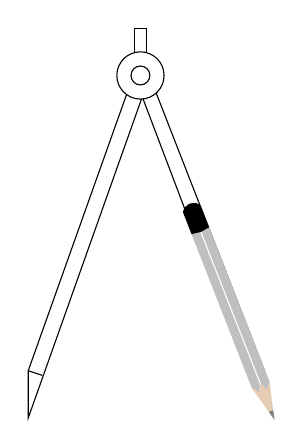
\begin{tikzpicture}
\begin{scope}[rotate=0,transform shape,scale=3]
\draw (2.95,3.7) rectangle (3,3.95);
\draw (2.92,3.68) -- (2.5,2.5) -- (2.5,2.3) -- (2.99,3.68);
\draw (3.5,2.5) -- (3.43,2.48) -- (2.975,3.68);
\draw (3.04,3.68) -- (3.5,2.5);
\draw (2.5,2.5) -- (2.56,2.48);
\draw[fill=white] (2.975,3.75) circle (0.1cm);
\draw (2.975,3.75) circle (0.04cm);
\end{scope}
\begin{scope}[xshift=10.34cm,yshift=7.28cm,rotate=21.4,scale=.6]          
\fill[gray!50] (0,4) -- (0.4,4) -- (0.4,0) --
               (0.3,-0.15) -- (0.2,0) -- (0.1,-0.14) --
               (0,0) -- cycle;
\draw[color=white] (0.2,4) -- (0.2,0);
\fill[black] (0,3.5) -- (0.2,3.47) -- (0.4,3.5) --
             (0.4,4) arc(30:150:0.23cm);
\fill[brown!40] (0,0) -- (0.2,-0.8)
    node[coordinate,pos=0.75](a){} -- 
    (0.4,0)node[coordinate,pos=0.25](b){} -- 
    (0.3,-0.15) -- (0.2,0) -- (0.1,-0.14) -- cycle;
\fill[gray] (a) -- (0.2,-0.8) -- (b) -- cycle;
\end{scope}
\end{tikzpicture}
}
\hfill
\rightfigure[c]
{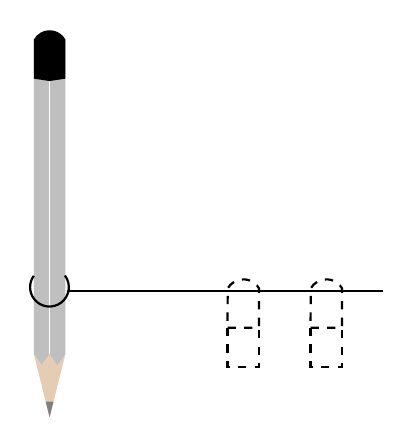
\begin{tikzpicture}[rotate=0,scale=1]          
\fill[gray!50] (0,4) -- (0.4,4) -- (0.4,0) --
               (0.3,-0.15) -- (0.2,0) -- (0.1,-0.14) --
               (0,0) -- cycle;
\draw[color=white] (0.2,4) -- (0.2,0);
\fill[black] (0,3.5) -- (0.2,3.47) -- (0.4,3.5) --
             (0.4,4) arc(30:150:0.23cm);
\fill[brown!40] (0,0) -- (0.2,-0.8)
    node[coordinate,pos=0.75](a){} -- 
    (0.4,0) node[coordinate,pos=0.25](b){} -- 
    (0.3,-0.15) -- (0.2,0) -- (0.1,-0.14) -- cycle;
\fill[gray] (a) -- (0.2,-0.8) -- (b) -- cycle;

\draw[thick] (0.395,1) arc (37:-216:7pt);
\coordinate (knot) at (0.44,.8);
\draw[thick] (knot) -- +(4,0);
\fill (knot) circle (.7pt);

\begin{scope}[xshift=100pt,yshift=-90pt]
\draw[dashed,thick] (0,3.5) -- (0.4,3.5) -- 
      (0.4,4) arc(30:150:0.23cm) -- cycle;
\draw[dashed,thick] (0,3.5) -- ++(0,-.5) -- ++(.4,0) -- ++(0,.5);
\end{scope}

\begin{scope}[xshift=70pt,yshift=-90pt]
\draw[dashed,thick] (0,3.5) -- (0.4,3.5) -- 
      (0.4,4) arc(30:150:0.23cm) -- cycle;
\draw[dashed,thick] (0,3.5) -- ++(0,-.5) -- ++(.4,0) -- ++(0,.5);
\end{scope}
\end{tikzpicture}
}
\leftcaption{A fixed compass. One leg has a needle that is placed at the center of the circle. A pencil attached to the other leg is used to draw the circle. The legs are joined by a tight hinge so that the distance between the legs (the radius of the circle) is maintained even when the compass is lifted from the paper.}\label{fig.fixed-compass}
\rightcaption{A collapsing compass. The user holds a piece of string at the center of the circle. The other end of the string is tied to a pencil and is used to draw the circle. When the compass is lifted from the paper, the fingers (dashed) can easily slip to a new position.}\label{fig.collapsing-compass}
\end{figure}

This chapter begins with a discussion of the relevance of studying construction with a straightedge and compass (Sect.~\ref{s.relevance}).
Section~\ref{s.collapse} compares the two types of compasses in the most elementary construction: a perpendicular bisector. Section~\ref{s.collapse-copy} presents Euclid's method of copying a line segment using a collapsing compass. This proves that any construction that can be done using a fixed compass can be performed using a collapsing compass. Section~\ref{s.collapse-copy-incorrect} shows a proof of this theorem which seems to be correct, but does not work for all configurations of lines and points. To emphasize that one must not trust diagrams, Sect.~\ref{s.collapse-isoceles} presents a famous alleged proof that all triangles are isoceles; the proof appears to be correct but is not because it is based on an incorrect diagram.

\section{Construction with a Straightedge and Compass}\label{s.relevance}

Construction with a straightedge and compass used to be the fundamental concept taught in Euclidean geometry. Recently, it has fallen out of favor in school curricula. It is certainly true that the topic has little, if any, practical use. As we show in Sects.~\ref{s.neusis}, \ref{s.neusis-doubling}, \ref{s.q}, \ref{s.square-quad}, the Greeks knew how to perform constructions that are impossible with a straightedge and compass by using tools only slightly more advanced. Today, using numerical methods, computers can perform constructions to any desired precision.

Nevertheless, I believe that there are advantages to studying constructions:
\begin{itemize}
\item It is more fun and more challenging to learn geometry through constructions than simply to read theorems and proofs.
\item Significant breakthroughs in mathematics have been achieved by attempts to find constructions. Chapter~\ref{c.heptadecagon} presents a construction by Gauss that led to modern abstract algebra, in particular, the theory developed by \'{E}variste Galois.\index{Galois, Evariste@Galois, \'{E}variste}
\item It is somewhat counterintuitive and therefore very interesting that it can be proved that it is impossible to construct some geometric objects.
\item Sadly, there a many people who waste years of their lives trying to perform impossible constructions. Students should certainly be aware of the futility of such efforts.
\end{itemize}

\section{Fixed Compasses and Collapsing Compasses}\label{s.collapse}

Some geometry textbooks present the construction of a perpendicular bisector\index{Collapsing compass!construction of a perpendicular bisector} of a line segment by constructing two circles centered at the ends of the line segment such that the radii are equal and \emph{greater than half the length of the segment} (Fig.~\ref{f.collapse-perp-bisector-fixed}). This can only be done with a fixed compass because after drawing the circle centered at $A$, the distance between the legs of the compass needs to remain fixed to draw the circle centered at $B$.

\begin{figure}[t]
\subfigures
\leftfigure[c]{
\begin{tikzpicture}[scale=0.5]
\coordinate (A) at (0,0);
\coordinate (B) at (4,0);
\vertex{A};
\vertex{B};
\draw (A) node[below left] {$A$} -- (B) node[below right] {$B$};
\draw[name path=larc] (A) ++(-60:3cm) arc (-60:60:3cm);
\draw[name path=rarc] (B) ++(-120:3cm) arc (-120:-240:3cm);
\path [name intersections={of=larc and rarc,by={b,t}}];
\node[above right,xshift=-2pt,yshift=5pt] at (t) {$C$};
\node[below left,xshift=2pt,yshift=-5pt] at (b) {$D$};
\draw ($ (b) ! 1.2 ! (t)$) -- ($ (t) ! 1.2 ! (b)$);
\end{tikzpicture}
}
\hfill
\rightfigure[c]{
\begin{tikzpicture}[scale=0.5]
\coordinate (A) at (0,0);
\coordinate (B) at (4,0);
\vertex{A};
\vertex{B};
\draw (A) node[below left] {$A$} -- (B) node[below right] {$B$};
\draw[name path=larc] (A) ++(-80:4cm) arc (-80:80:4cm);
\draw[name path=rarc] (B) ++(-100:4cm) arc (-100:-260:4cm);
\path [name intersections={of=larc and rarc,by={b,t}}];
\node[above right,xshift=-2pt,yshift=3pt] at (t) {$C$};
\node[below left,xshift=2pt,yshift=-3pt] at (b) {$D$};
\draw ($ (b) ! 1.2 ! (t)$) -- ($ (t) ! 1.2 ! (b)$);
\end{tikzpicture}
}
\leftcaption{Construction of a perpendicular bisector with a fixed compass}\label{f.collapse-perp-bisector-fixed}
\rightcaption{Construction of a perpendicular bisector with a collapsing compass}\label{f.collapse-perp-bisector-collapse}
\end{figure}

Figure~\ref{f.collapse-perp-bisector-collapse} shows the construction of a perpendicular bisector with a collapsing compass by constructing two circles: one centered at $A$ with radius $\overline{AB}$ and one centered at $B$ with radius $\overline {BA}$. This can be done with a collapsing compass because (obviously) $\overline{AB}=\overline{BA}$, so the compass does not have to ``remember'' the length of $\overline{AB}$ to construct a circle centered at $B$ with the same radius.
The proof that the line constructed shown in Fig.~\ref{f.collapse-perp-bisector-fixed} is a perpendicular bisector is not at all elementary because relatively advanced concepts like congruent triangles have to be used. However, the proof that the construction of a perpendicular bisector shown in Fig.~\ref{f.collapse-perp-bisector-collapse} is correct is simple and based on the fact that $\triangle ABC$ is an equilateral triangle. In fact, that is the first proposition in Euclid's \textit{Elements}.\index{Euclid's elements@Euclid's \textit{Elements}}
$\overline{AC}=\overline{AB}$ since they are radii of the same circle and, similarly, $\overline{BC}=\overline{BA}$. We have: $
\overline{AC}=\overline{AB}=\overline{BA}=\overline{BC}$.

Figure~\ref{f.collapse-equilateral-fixed} shows that for the construction with a fixed compass, the triangle will be isosceles, not necessarily an equilateral triangle as in \index{Collapsing compass!construction of an equilateral triangle} Euclid's first proposition (Fig.~\ref{f.collapse-equilateral-collapse}).

\begin{figure}[b]
\subfigures
\leftfigure[c]{
\begin{tikzpicture}[scale=0.5]
\coordinate (A) at (0,0);
\coordinate (B) at (4,0);
\vertex{A};
\vertex{B};
\draw (A) node[below left] {$A$} -- (B) node[below right] {$B$};
\draw[name path=larc] (A) ++(-60:3cm) arc (-60:60:3cm);
\draw[name path=rarc] (B) ++(-120:3cm) arc (-120:-240:3cm);
\path [name intersections={of=larc and rarc,by={b,t}}];
\vertex{t};
\vertex{b};
\node[above right,xshift=-2pt,yshift=5pt] at (t) {$C$};
\node[below left,xshift=2pt,yshift=-5pt] at (b) {$D$};
\draw (A) -- (t);
\draw (B) -- (t);
\end{tikzpicture}
}
\hfill
\rightfigure[c]{
\begin{tikzpicture}[scale=0.5]
\coordinate (A) at (0,0);
\coordinate (B) at (4,0);
\draw (A) node[below left] {$A$} -- (B) node[below right] {$B$};
\vertex{A};
\vertex{B};
\draw[name path=larc] (A) ++(-80:4cm) arc (-80:80:4cm);
\draw[name path=rarc] (B) ++(-100:4cm) arc (-100:-260:4cm);
\path [name intersections={of=larc and rarc,by={b,t}}];
\vertex{t};
\vertex{b};
\node[above right,xshift=-2pt,yshift=3pt] at (t) {$C$};
\node[below left,xshift=2pt,yshift=-3pt] at (b) {$D$};
\draw (A) -- (t);
\draw (B) -- (t);
\end{tikzpicture}
}
\leftcaption{Construction of an isoceles triangle with a fixed compass}\label{f.collapse-equilateral-fixed}
\rightcaption{Construction of an equilateral triangle with a collapsing compass}\label{f.collapse-equilateral-collapse}
\end{figure}

\section{Euclid's Construction for Copying a Line Segment}\label{s.collapse-copy}

The second proposition of  Euclid's \textit{Elements}\index{Euclid's elements@Euclid's \textit{Elements}} shows how to copy a given line segment $\overline{AB}$ to a segment of the same length, one of whose end points is a given point $C$. Therefore, a fixed compass adds no additional capabilities and a collapsing compass is sufficient, although constructions are easier with a fixed compass.

\begin{theorem}
Given a line segment $\overline{AB}$ and a point $C$, a line segment $\overline{CC'}$, one of whose endpoints is $C$, can be constructed using a collapsing compass, such that $\overline{AB}=\overline{CC'}$ (Fig.~\ref{f.collapse-copying-1}).
\end{theorem}

\begin{figure}[t]
\subfigures
\leftfigure[c]{
\begin{tikzpicture}[scale=0.5]
\coordinate (C) at (0,0);
\coordinate (A) at (3,0);
\draw (A) node[below,xshift=-2pt,yshift=-2pt] {$A$} -- +(40:4) coordinate (B) node[right] {$B$};
\vertex{A};
\vertex{B};
\vertex{C};
\node[below,xshift=2pt,yshift=-2pt] at (C) {$C$};
\draw[thick,dashed] (C) -- +(160:4) coordinate (D) node[below] {$C'$};
\vertex{D};
\end{tikzpicture}
}
\hfill
\rightfigure[c]{
\begin{tikzpicture}[scale=0.5]
\coordinate (C) at (0,0);
\coordinate (A) at (3,0);
\draw (A) node[below,xshift=-2pt,yshift=-2pt] {$A$} -- +(40:4) coordinate (B) node[right] {$B$};
\vertex{B};
\node[below,xshift=2pt,yshift=-2pt] at (C) {$C$};
\draw (A) -- (C);
\path[name path=larc] (C) ++(-70:2.5cm) arc (-70:70:2.5cm);
\path[name path=rarc] (A) ++(-110:2.5cm) arc (-110:-250:2.5cm);
\path [name intersections={of=larc and rarc,by={d,D}}];
\node[above] at (D) {$D$};
\draw (A) -- (D);
\draw (C) -- (D);
\end{tikzpicture}
}
\leftcaption{Copy the line segment $\overline{AB}$. The orientation of $\overline{CC'}$ is not important.}\label{f.collapse-copying-1}
\rightcaption{Copying a line segment with a collapsing compass}\label{f.collapse-copying-2}
\end{figure}

\begin{proof}
Construct the line segment $\overline{AC}$. Construct the equilateral triangle $\triangle ACD$ whose base is $\overline{AC}$ (Fig.~\ref{f.collapse-copying-2}). By Euclid's first proposition, the triangle can be constructed using a collapsing compass. Construct the ray that is an extension of the line segment \emph{from $D$ to $A$}, and construct the ray that is an extension of the line segment \emph{from $D$ to $C$} (Fig.~\ref{f.collapse-copying-3}). Construct the circle centered at $A$ with radius $\overline{AB}$ and denote the intersection of the circle and the ray extending $\overline{DA}$ by $E$. Construct the circle centered at $D$ with radius $\overline{DE}$ and denote the intersection of the circle and the ray extending $\overline{DC}$ by $F$ (Fig.~\ref{f.collapse-copying-4}).

\begin{figure}[b]
\subfigures
\leftfigure[c]{
\begin{tikzpicture}[scale=0.4]
\coordinate (C) at (0,0);
\coordinate (A) at (3,0);
\draw (A) node[below,xshift=-2pt,yshift=-2pt] {$A$} -- +(40:4) coordinate (B) node[right] {$B$};
\node[below,xshift=2pt,yshift=-2pt] at (C) {$C$};
\draw (A) -- (C);
\path[name path=larc] (C) ++(-70:2.5cm) arc (-70:70:2.5cm);
\path[name path=rarc] (A) ++(-110:2.5cm) arc (-110:-250:2.5cm);
\path [name intersections={of=larc and rarc,by={d,D}}];
\node[above] at (D) {$D$};
\draw (A) -- (D);
\draw (C) -- (D);
\draw[name path=ray2] (D) -- ($ (D) ! 3 ! (C) $);
\draw[name path=ray1] (D) -- ($ (D) ! 3 ! (A) $);
\end{tikzpicture}
}
\hfill
\rightfigure[c]{
\begin{tikzpicture}[scale=0.4]
\coordinate (C) at (0,0);
\coordinate (A) at (3,0);
\draw (A) node[below,xshift=-2pt,yshift=-2pt] {$A$} -- +(40:4) coordinate (B) node[right] {$B$};
\node[below,xshift=2pt,yshift=-2pt] at (C) {$C$};
\draw (A) -- (C);
\path[name path=larc] (C) ++(-70:2.5cm) arc (-70:70:2.5cm);
\path[name path=rarc] (A) ++(-110:2.5cm) arc (-110:-250:2.5cm);
\path [name intersections={of=larc and rarc,by={d,D}}];
\node[above] at (D) {$D$};
\draw (A) -- (D);
\draw (C) -- (D);
\draw[name path=ray2] (D) -- ($ (D) ! 3 ! (C) $);
\draw[name path=ray1] (D) -- ($ (D) ! 3 ! (A) $);
\node[draw,circle through=(B),name path=c1] at (A) {};
\path [name intersections={of=c1 and ray1,by={E,e}}];
\node[right,xshift=2pt,yshift=-2pt] at (E) {$E$};
\end{tikzpicture}
}
\leftcaption{Constructing rays from $D$}\label{f.collapse-copying-3}
\rightcaption{Constructing a circle with radius $\overline{AB}$}\label{f.collapse-copying-4}
\end{figure}
$\overline{DC}=\overline{DA}$ because $\triangle ACD$ is equilateral. $\overline{AE}=\overline{AB}$ are radii of the same circle, as are $\overline{DF}=\overline{DE}$. Therefore:
\[
\overline{CF}=\overline{DF}-\overline{DC}=\overline{DE}-\overline{DC}=\overline{DE}-\overline{DA}=\overline{AE}=\overline{AB}\,.
\]
\end{proof}

\begin{figure}
\begin{center}
\begin{tikzpicture}[scale=0.4]
\clip (-5,-4.5) rectangle (8,6);
\coordinate (C) at (0,0);
\coordinate (A) at (3,0);
\draw (A) node[below,xshift=-2pt,yshift=-2pt] {$A$} -- +(40:4) coordinate (B) node[right] {$B$};
\node[below,xshift=2pt,yshift=-2pt] at (C) {$C$};
\draw (A) -- (C);
\path[name path=larc] (C) ++(-70:2.5cm) arc (-70:70:2.5cm);
\path[name path=rarc] (A) ++(-110:2.5cm) arc (-110:-250:2.5cm);
\path [name intersections={of=larc and rarc,by={d,D}}];
\node[above] at (D) {$D$};
\draw (A) -- (D);
\draw (C) -- (D);
\draw[name path=ray2] (D) -- ($ (D) ! 3 ! (C) $);
\draw[name path=ray1] (D) -- ($ (D) ! 3 ! (A) $);
\node[draw,circle through=(B),name path=c1] at (A) {};
\path [name intersections={of=c1 and ray1,by={E,e}}];
\node[right,xshift=2pt,yshift=-2pt] at (E) {$E$};
\node[draw,circle through=(E),name path=c2] at (D) {};
\path [name intersections={of=c2 and ray2,by={F,f}}];
\node[left,xshift=-2pt,yshift=-2pt] at (F) {$F$};
\path (A) -- node[right] {$a$} (E);
\path (C) -- node[left] {$a$} (F);
\draw[white,fill=white] (-5,4.5) rectangle +(13,1.5);
\end{tikzpicture}
\end{center}
\caption{Construction of $\overline{CF}=\overline{AB}$}\label{f.collapse-copying-5}
\end{figure}

The specification of the directions of the rays is essential. The proof here works for any line segment $\overline{AB}$ and any point $C$, regardless of its position relative to $\overline{AB}$.  By specifying directions the ``cone'' enclosed by the two rays will intersect the circles even if $\overline{AC}>\overline{AB}$ (Fig.~\ref{f.collapse-copying-6}).

\begin{figure}
\begin{center}
\begin{tikzpicture}[scale=0.4]
\clip (-12,-6) rectangle (11,10);
\coordinate (C) at (-4,0);
\coordinate (A) at (3,0);
\draw (A) node[below,xshift=-2pt,yshift=-2pt] {$A$} -- +(40:4) coordinate (B) node[right] {$B$};
\node[below,xshift=2pt,yshift=-2pt] at (C) {$C$};
\draw (A) -- (C);
\path[name path=larc] (C) ++(-70:7cm) arc (-70:70:7cm);
\path[name path=rarc] (A) ++(-110:7cm) arc (-110:-250:7cm);
\path [name intersections={of=larc and rarc,by={d,D}}];
\node[above] at (D) {$D$};
\draw (A) -- (D);
\draw (C) -- (D);
\draw[name path=ray2] (D) -- ($ (D) ! 2 ! (C) $);
\draw[name path=ray1] (D) -- ($ (D) ! 2 ! (A) $);
\node[draw,circle through=(B),name path=c1] at (A) {};
\path [name intersections={of=c1 and ray1,by={e,E}}];
\node[right,xshift=2pt,yshift=-2pt] at (E) {$E$};
\node[draw,circle through=(E),name path=c2] at (D) {};
\path [name intersections={of=c2 and ray2,by={F,f}}];
\node[left,xshift=-2pt,yshift=-2pt] at (F) {$F$};
\path (A) -- node[right] {$a$} (E);
\path (C) -- node[left] {$a$} (F);
\draw[white,fill=white] (-12,8) rectangle +(23,2);
\end{tikzpicture}
\end{center}
\caption{Construction for $\overline{AC}>\overline{AB}$}\label{f.collapse-copying-6}
\end{figure}

%%%%%%%%%%%%%%%%%%%%%%%%%%%%%%%%%%%%%%%%%%%%%%%%%%%%%%%%%%%%%%%

\section{A Flawed Construction for Copying a Line Segment}\label{s.collapse-copy-incorrect}

\begin{proof}
Construct three circles: one centered at $A$ with radius $\overline{AB}$, one centered at $A$ with radius $\overline{AC}$, and one centered at $C$ with radius $\overline{AC}=\overline{CA}$. Denote the intersections of the circles centered at $A$ and $C$ by $E$ and $F$, and denote an intersection of the circle centered at $C$ and the circle centered at $A$ with radius $\overline{AB}$ by $D$. If $\overline{AC}>\overline{AB}$, the construction is as shown in Fig.~\ref{f.collapse-incorrect-1}.
\begin{figure}[t]
\begin{center}
\begin{tikzpicture}[scale=0.5]
\coordinate (C) at (-2,0);
\coordinate (A) at (2.5,0);
\coordinate (B) at (4.5,1.5);
\draw (A) node[below right] {$A$} -- (B) node[right] {$B$};
\node[left,xshift=-2pt] at (C) {$C$};
\node[draw,circle through=(B),name path=c1] at (A) {};
\node[draw,circle through=(C),name path=c2] at (A) {};
\node[draw,circle through=(A),name path=c3] at (C) {};
\path [name intersections={of=c1 and c3,by={D,f}}];
\path [name intersections={of=c2 and c3,by={E,F}}];
\node[below right,xshift=4pt] at (D) {$D$};
\node[above,yshift=2pt] at (E) {$E$};
\node[below,yshift=-2pt] at (F) {$F$};
\vertex{C};
\end{tikzpicture}
\end{center}
\caption{Flawed construction for copying a line segment (1)}\label{f.collapse-incorrect-1}
\end{figure}

\begin{figure}[t]
\begin{center}
\begin{tikzpicture}[scale=0.5]
\clip (-8,-1) rectangle (9,5);
\coordinate (C) at (-2,0);
\coordinate (A) at (2.5,0);
\coordinate (B) at (4.5,1.5);
\draw[thick] (A) node[below right] {$A$} -- (B) node[right] {$B$};
\vertex{A};
\vertex{C};
\node[below left] at (C) {$C$};
\node[draw,circle through=(B),name path=c1] at (A) {};
\node[draw,circle through=(C),name path=c2] at (A) {};
\node[draw,circle through=(A),name path=c3] at (C) {};
\path [name intersections={of=c1 and c3,by={D,f}}];
\path [name intersections={of=c2 and c3,by={E,F}}];
\node[draw,circle through=(D),name path=c4] at (E) {};
\path [name intersections={of=c2 and c4,by={g,G}}];
\node[left] at (G) {$G$};
\node[below right,yshift=2pt,xshift=2pt] at (D) {$D$};
\node[above] at (E) {$E$};
\vertex{E};
\vertex{F};
\draw (C) -- (G);
\draw (A) -- (G) -- (E) -- (C) -- (D);
\draw (A) -- (D) -- (E) -- cycle;
\end{tikzpicture}
\end{center}
\caption{Flawed construction for copying a line segment (2)}\label{f.collapse-incorrect-2}
\end{figure}

Construct a circle centered at $E$ with radius $\overline{ED}$. Denote the intersection of this circle with the circle centered at $A$ with radius $\overline{AC}$ by $G$. There are two intersections, so choose the one closer to $C$ (Fig.~\ref{f.collapse-incorrect-2}).
$\overline{CD}=\overline{CE}$ are radii of the same circle as are $\overline{AE}=\overline{AG}$. By construction the radii $\overline{CE}$ and $\overline{AE}$ are equal. Therefore,
\[
\overline{CD} = \overline{CE} = \overline{AE} = \overline{AG}\,.
\]
$\overline{EG} = \overline{ED}$ are radii of the same circle, so $\triangle EAG\cong \triangle DCE$ by side-side-side and $\angle GEA = \angle DEC$.

Since:
\[
\angle GEC = \angle GEA \!-\!\angle CEA = \angle DEC\!-\!\angle CEA = \angle DEA\,,
\] it follows that $\triangle ADE\cong\triangle CGE$ by side-angle-side. $\overline{AB}=\overline{AD}$ are radii of the smaller circle centered at $A$, so $\overline{GC}=\overline{AD}=\overline{AB}$.
\end{proof}

The proof is correct only if $\overline{AC}>\overline{AB}$.  Figure~\ref{f.collapse-incorrect-4} shows a diagram where $\overline{AC}<\overline{A}B$ and you can see that $\overline{AB}\neq\overline{GC}$.

\begin{figure}[t]
\begin{center}
\begin{tikzpicture}[scale=0.5]
\coordinate (C) at (-1,0);
\coordinate (A) at (2,0);
\coordinate (B) at (6,1.5);
\draw[thick] (A) node[below right] {$A$} -- (B) node[right] {$B$};
\node[left,xshift=-2pt] at (C) {$C$};
\node[draw,circle through=(B),name path=c1] at (A) {};
\node[draw,circle through=(C),name path=c2] at (A) {};
\node[draw,circle through=(A),name path=c3] at (C) {};
\path [name intersections={of=c1 and c3,by={D,f}}];
\path [name intersections={of=c2 and c3,by={E,F}}];
\node[above left,xshift=4pt] at (D) {$D$};
\node[above,yshift=2pt] at (E) {$E$};
\node[below,yshift=-2pt] at (F) {$F$};
\vertex{A};
\vertex{C};
\node[draw,circle through=(D),name path=c4] at (E) {};
\path [name intersections={of=c2 and c4,by={g,G}}];
\node[right,xshift=2pt,yshift=2pt] at (G) {$G$};
\draw[thick] (G) -- (C);
\end{tikzpicture}
\end{center}
\caption{A diagram for which the proof doesn't work}\label{f.collapse-incorrect-4}
\end{figure}

\newpage

\section{Don't Trust a Diagram}\label{s.collapse-isoceles}

\begin{theorem}[Incorrect, of course]
All triangles are isosceles.
\end{theorem}\index{Triangle!isoceles@all are isoceles}

\begin{proof}[Incorrect]
Given an arbitrary triangle $\triangle ABC$, let $P$ be the intersection of the angle bisector of $\angle BAC$ and the perpendicular bisector of $\overline{BC}$. The intersections of the altitudes from $P$ to the sides $\overline{AB}$, $\overline{AC}$ are denoted by $E,F$ (Fig.~\ref{f.collapse-isoceles-1}). 
\begin{figure}[t]
\begin{center}
\begin{tikzpicture}[scale=1.1]
\coordinate (P) at (0,0);
\node[xshift=4mm,yshift=1mm] at (P) {$P$};
\coordinate [label=left:$B$] (B)  at (-2,-2);
\coordinate [label=right:$C$] (C)  at (4,-2);
\coordinate [label=above:$A$] (A)  at (-1,2);
\node[below,yshift=-12pt,xshift=1pt] at (A) {$\alpha$};
\node[below,yshift=-12pt,xshift=13pt] at (A) {$\alpha$};
\draw (A) -- (B);
\draw (A) -- (C);
\draw (B) -- (C);
\draw (A) -- (P);
\draw (B) -- (P);
\draw (C) -- (P);
\coordinate[label=left:$E$] (E) at ($ (A) ! .44 ! (B) $);
\draw[rotate=-100] (E) rectangle +(6pt,6pt);
\draw (P) -- (E);
\coordinate (F) at ($ (A) ! .33 ! (C) $);
\node[right,xshift=2pt,yshift=2pt] at (F) {$F$};
\draw[rotate=-132] (F) rectangle +(6pt,6pt);
\draw (P) -- (F);
\coordinate[label=below:$D$] (D) at ($ (B) ! .33 ! (C) $);
\draw (D) rectangle +(6pt,6pt);
\draw (P) -- (D);
\node[left] at ($ (A) ! .5 ! (E) $) {};
\node[left] at ($ (B) ! .5 ! (E) $) {};
\node[below] at ($ (B) ! .5 ! (D) $) {$a$};
\node[below] at ($ (C) ! .5 ! (D) $) {$a$};
\node[right,xshift=2pt] at ($ (A) ! .5 ! (F) $) {};
\node[right,xshift=2pt] at ($ (C) ! .5 ! (F) $) {};
\vertex{P};
\end{tikzpicture}
\end{center}
\caption{An incorrect proof that all triangles are isoceles}\label{f.collapse-isoceles-1}
\end{figure}
$\triangle APE\cong \triangle APF$ because they are right triangles with equal angles $\alpha$ and common side $\overline{AP}$. $\triangle DPB\cong \triangle DPC$ since they are right triangles, $\overline{PD}$ is a common side and $\overline{BD}=\overline{CD}=a$. $\triangle EPB\cong \triangle FPC$ since they are right triangles, $\overline{EP}=\overline{PF}$ by the first congruence and $\overline{PB}=\overline{PC}$ by the second congruence. By combining the equations we get that $\triangle ABC$ is isoceles:
\[
\overline{AB}= \overline{AE}+\overline{EB}=\overline{AF}+\overline{FC} =\overline{AC}\,.
\]
\end{proof}

The \emph{logic} of the proof is correct, but the diagram upon which the proof is based is not correct because point $P$ is \emph{outside} the triangle (Fig.~\ref{f.collapse-isoceles-2}).

\begin{figure}[t]
\begin{center}
\begin{tikzpicture}[scale=.7]
\coordinate (B) at (0,0);
\coordinate (C) at (8,0);
\path[name path=ba] (B) -- +(70:6);
\path[name path=ca] (C) -- +(140:8.5);
\path [name intersections={of=ba and ca,by={A}}];
\draw (B) -- (C) -- (A) -- cycle;
\node[above] at (A) {$A$};
\node[below,yshift=-12pt,xshift=-1pt] at (A) {$\alpha$};
\node[below right,xshift=5pt,yshift=-12pt] at (A) {$\alpha$};
\node[left] at (B) {$B$};
\node[right] at (C) {$C$};
\draw[name path=angle] (A) -- +(-75:9);
\draw ($(B)!.5!(C)$) -- +(0,3);
\draw[name path=perp] ($(B)!.5!(C)$) -- +(0,-3.5);
\path [name intersections={of=angle and perp,by={X}}];
\vertex{X};
\draw (4,0) rectangle +(10pt,10pt);
\node[right] at (X) {$P$};
\end{tikzpicture}
\end{center}
\caption{Why the construction doesn't work}\label{f.collapse-isoceles-2}
\end{figure}


\newpage

\subsection*{What Is the Surprise?}

As a student I took it for granted that a compass has a friction joint that maintains the distance between the point and the pencil when it is lifted from the paper. When the teacher used a compass made from a piece of string and a piece of chalk, I never imagined that it differed from my compass. The article by Gotfried Toussaint was a real surprise, as was his demonstration that post-Euclid proofs were incorrect because they depended on diagrams that made unwarranted assumptions. I recommend the article to readers who wish to deepen their understanding of  proofs in mathematics.

\subsection*{Sources}

This chapter is based on \cite{toussaint}. The incorrect construction of the equivalence of the two compasses in Sect.~\ref{s.collapse-copy-incorrect} is from \cite{rusty}. A comprehensive English translation of Euclid's \textit{Elements} together with an extensive commentary \cite{euclid} was written by Thomas L. Heath\index{Heath, Thomas L.}, one of the foremost experts in Greek mathematics.
